% !TEX root = ../main.tex

\section{Implicit Differentiation}
Some curves' equations can't be solved for y (or maybe not easily), but we should still be able find the tangent line and its slope.
\begin{example}
    \begin{equation*}
        x^2 + y^2 = 4
    \end{equation*}
    \begin{itemize}
        \item Not a function!
        \item Can solve for $y$
    \end{itemize}
    \begin{equation*}
        y = \pm \sqrt{4 - x^2}
    \end{equation*}
    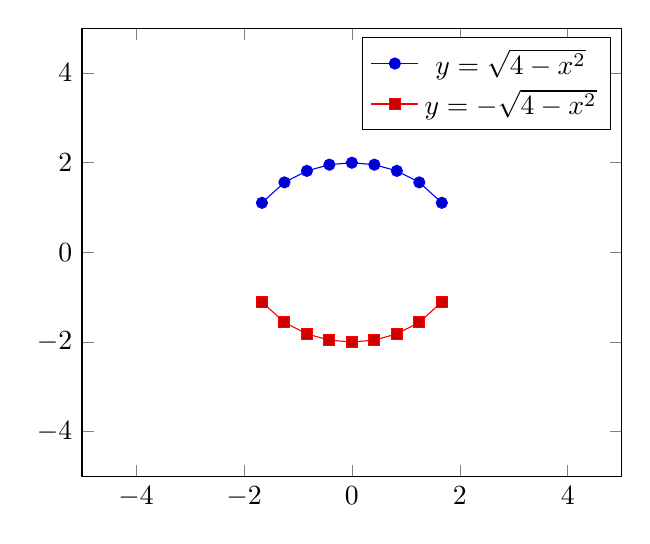
\begin{tikzpicture}
        \begin{axis}[xmin = -5, xmax=5, ymin=-5, ymax=5]
            \addplot +[blue]{sqrt(4 - x^2)};
            \addplot +[red]{-sqrt(4 - x^2)};
            \legend{$y = \sqrt{4 - x^2}$, $y = -\sqrt{4 - x^2}$};
        \end{axis}
    \end{tikzpicture}
    Given an expression with $x$s and $y$s to find $\deriv[y]$
    \begin{enumerate}
        \item Treat $y$ as a function of $x$ and differentiate both sides of the equation with respect to $x$
        \item Solve for $\deriv[y]$
        \item Win
    \end{enumerate}
\end{example}
\begin{note}
    When doing step one (1), you can think ``Whenever I thake the derivative of $y$ multiply that term by $\deriv[y]$.''
\end{note}
\begin{example}
    If $x^2 + y^2 = 4$ use implicit differentiation to find $\deriv[y]$
    \begin{enumerate}[a\symbol{41}] % \symbol is used rather than `)' so chktex does not freak out
        \item \begin{gather*}
            \deriv \left(x^2 + y^2\right) = \deriv \left(4\right) \\
            2x + 2y\deriv[y] = 0 \\
            \dfrac{\cancel{2y}\deriv[y]}{\cancel{2y}} = \dfrac{-2x}{2y} \\
            \deriv[y] = \dfrac{-2x}{2y} \\
            \deriv[y] = -\dfrac{x}{y}
        \end{gather*}
        \item Find the slope of the tangent line at $\left(1, \sqrt{3}\right)$ \\
        \begin{equation*}
            \Eval{\deriv[y]}{\left(1, \sqrt{3}\right)} = - \dfrac{1}{\sqrt{3}}
        \end{equation*}
        \begin{note}
            The line after $\deriv[y]$ is read as ``$\deriv[y]$ evaluated with $ x= 1$ and $y = \sqrt{3}$''
        \end{note}
        \item What is the equation of the tangent at $\left(1, \sqrt{3}\right)$
        \begin{gather*}
            y - y_1 = m\left(x - x_1\right) \\
            y - \sqrt{3} = - \dfrac{1}{\sqrt{3}}\left(x - 1\right)
        \end{gather*}
    \end{enumerate}
\end{example}
%TODO complete Section 3.2
